\begin{figure}
    \centering
    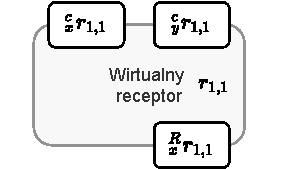
\includegraphics[width=0.75\columnwidth]{figures/ISR-vr-camera-model.pdf}
    \label{fig:model-vr-camera}
    \caption{Struktura ogólna wirtualnego receptora kamery RGB-D}
\end{figure}

\begin{figure}
    \centering
    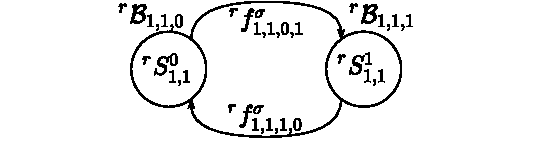
\includegraphics[width=\columnwidth]{figures/ISR-vr-camera-behaviours.pdf}
    \label{fig:zachowania-vr-camera}
    \caption{Automat zachowań wirtualnego receptora kamery RGB-D}
\end{figure}

Receptor wirtualny kamery RGBD (slajdy 120-122):
\begin{itemize}
    \item bufor wejściowy od rzeczywistego receptora: obraz z kamery,
    \item bufor wyjściowy do podsystemu sterowania
\end{itemize}


Zachowania:
\begin{itemize}
    \item ${}^{r}\mathcal{B}_{1,1,0}$ - detect blocks,
    \item ${}^{r}\mathcal{B}_{1,1,1}$ - detect places.
\end{itemize}